\section{Results}
\label{sec:Results}

\begin{figure}[t]
	\centering
	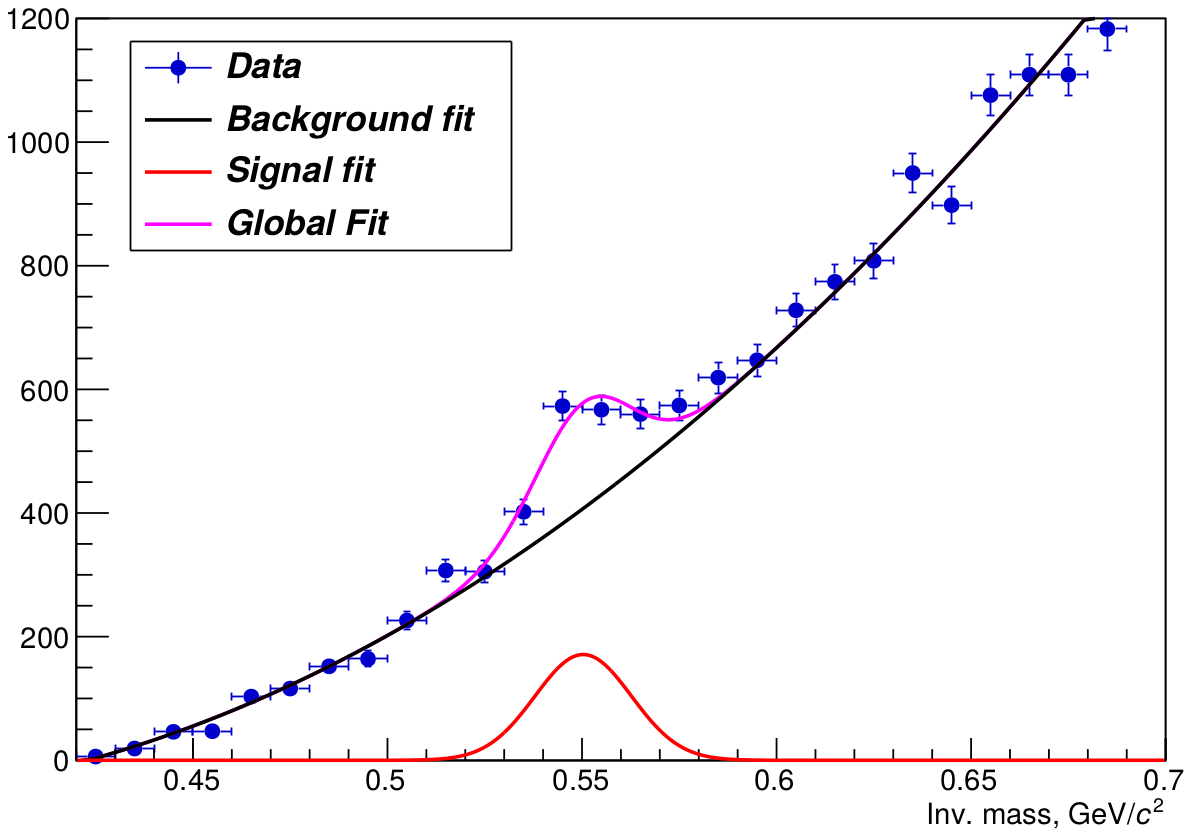
\includegraphics[width=0.55\textwidth]{Figures/EtaPeak500MeVlegscut.png}
	\caption{Invariant mass spectrum of $\pi^0\pi^{+}\pi^{-}$ after applying a momentum cut of 500 MeV on both legs. A peak can be seen where we expect the $\eta$ with a mass of $m_{\eta} = 547.862 \pm 0.017$ MeV \cite{PDG2018}; fitting the peak with a Gaussian gives a mass of $m_{\eta} = 550.3 \pm 1.8$ MeV and a width of $\Gamma_{\eta} = 12.4 \pm 2.7$ MeV with an estimated significance of 9.6$\sigma$}
	\label{fig:alpha}
\end{figure}

\begin{figure}[b]
	\centering
	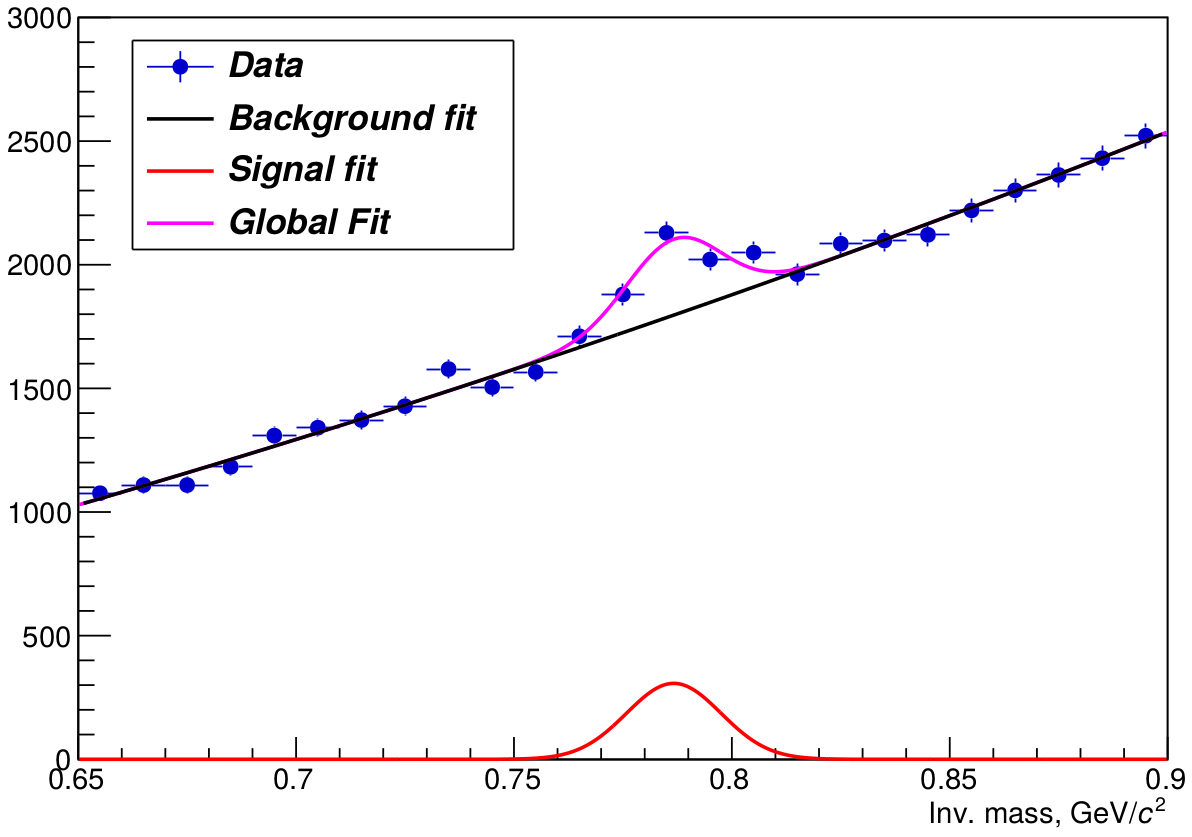
\includegraphics[width=0.55\textwidth]{Figures/OmegaPeak500MeVlegscut.png}
	\caption{Invariant mass spectrum of $\pi^0\pi^{+}\pi^{-}$ after applying a momentum cut of 500 MeV on both legs. A peak can be seen where we expect the $\omega$ with a mass of $m_{\omega} = 782.65 \pm 0.12$ MeV; fitting the peak with a Gaussian gives a mass of $m_{\omega} = 786.7 \pm 1.7$ MeV and a width of $\Gamma_{\omega} = 10.9 \pm 2.0$ MeV with an estimated significance of 4.9$\sigma$}
	\label{fig:alpha}
\end{figure}



show $\rho$ peak which is by-product in charged pi-pi spectrum from 3pi $a_1$ channel. Try to properly fit with fitting script. might be difficult because of weird background, has already been measured in ALICE, e.g. \cite{ALICErho}. \\